
\section{Compressed Air Equivalent}%
\label{sec:air design}%
The hydrogen part of the power generation and feed system consists of three main components: the fuel cell, the flow control unit, and the cool gas generator. In the air equivalent system, the fuel cell and CGG are replaced by subsystems that let through air at the same rate and pressure as the fuel cell and CGG would. The flow control unit is used as-is, controlling the flow of air instead of hydrogen. The system is depicted schematically in figure~\ref{fig:air test}. A picture of the realised test setup is shown in figure~\ref{fig:rl air test}.

\begin{figure}[htp]
    \centering
    \scalebox{0.8}{
        \begin{tikzpicture}[node distance=2 cm]
            % \draw[help lines] (0, -3) grid (10,3);
            \airsupply{origin}
            \draw[thick, densely dotted] (1, -1.5) -| +(4, 3.5) -| ++(0, 0);
            \node (airsupplytext) at (3, -2) {Air Supply};

            \aircgg{airsupply}
            \draw[thick, densely dotted] (aircgg) ++(0.75, -1.5) -| +(-5.5, 3.5) -| ++(0, 0);
            \node (airsupplytext) at (8, -2) {CGG Air Equivalent};

            \node[pressure regulator, right of=aircgg] (pregulator) {};
            \draw[thick] (aircgg) -- (pregulator);

            \airfc{pregulator}
            \draw[thick, densely dotted] (airfc) ++(0.75, -1) -| +(-4.5, 8) -| ++(0, 0);
            \node (airsupplytext) at (15.5, -4) {Fuel Cell Air Equivalent};

        \end{tikzpicture}
    }
    \caption{Fluidics of the Air Test Setup}%
    \label{fig:air test}%
\end{figure}

\begin{figure}
    \centering
    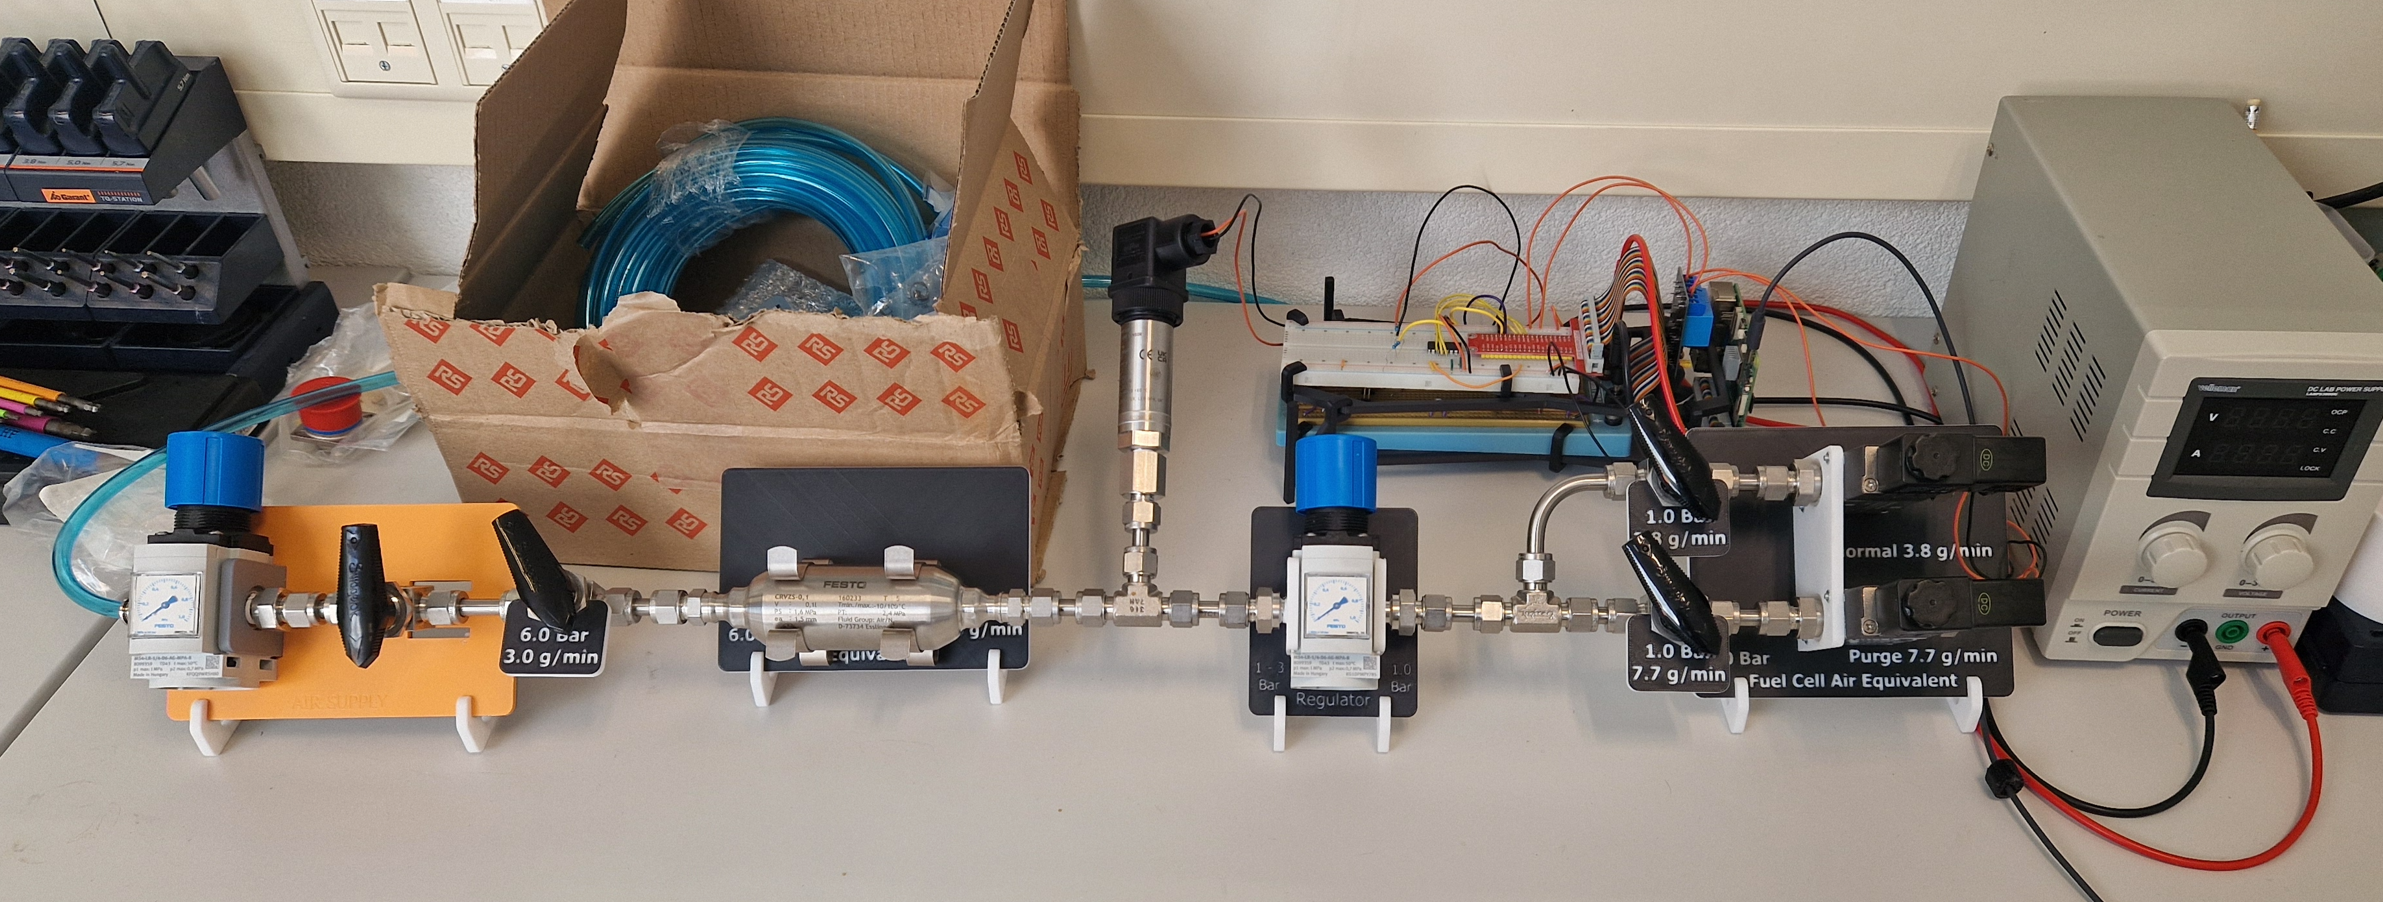
\includegraphics[width=\textwidth]{media/rl Air Setup.png}
    \caption{Picture of the Compressed Air Equivalent Test Setup}
    \label{fig:rl air test}
\end{figure}

\subsection*{CGG Equivalent}
The CGG produces hydrogen at a fixed rate regardless of output pressure. To simulate this, an orifice has been sized to the expected mass flow of the CGG. To ensure that this flow rate does not change with pressure, sonic flow must occur in the orifice. This occurs when the upstream pressure is at least 2 times the downstream pressure. The maximum expected CGG output pressure is 3 Bar, so the upstream pressure is set to 6 Bar to ensure sonic flow. The hydrogen that the CGG produces is stored in the internal volume of the CGG, which is approximately 0.1 L. Therefore, the air system includes a buffer volume of 0.1 L to simulate the CGG storage. The CGG equivalent also includes a pressure sensor to measure the pressure inside the buffer volume.

\subsection*{Fuel Cell Equivalent}
The fuel cell normally uses hydrogen at a rate that depends on power draw and at an increased rate during purge events. For the air tests, the `power draw' is assumed to be a fixed value of 200 W, which corresponds to a hydrogen mass flow of approximately 0.18 g/min. During purge events, the hydrogen mass flow is expected to increase to approximately 0.27 g/min. To simulate this with compressed air, two orifices have been sized to these flow rates at a pressure of 1 Bar, which corresponds to the operating pressure of the fuel cell. Solenoid valves are used to switch between the two orifices to simulate purge events.

Solenoid valves use a small amount of air to perform the switching operation. The solenoid itself operates a pilot valve, which then directs pressurised air to operate the main valve. This allows the solenoid valve to operate at higher pressures and still require quite little power to operate. This does however mean that a small amount of air is released to the atmosphere each time the valve switches. To ensure this does not affect the flow rates, it was considered to place the orifices before the valves. However, due to the way the valves operate, they require a small amount of back pressure to switch properly. When the orifices are placed before the valves, the output of the valve would be exposed to atmospheric pressure which is insufficient to allow the valve to operate properly.

The amount of air lost each time has been determined to be at most 1 microgram. This means the air lost during switching is insignificant for this test purpose, so long as the switch is not operated excessively.

As the fuel cell requires an input pressure of exactly 1 Bar, but the CGG volume can fluctuate between 1 and 4 Bar, a pressure regulator is used to ensure the fuel cell equivalent always receives air at 1 Bar. In the hydrogen system, this function will be performed by Stellar Space Industries' flow control system. However, as this system is not yet available, a commercial off-the-shelf pressure regulator is used for the air tests.

\subsection*{Control System}
The goal of the control system is to maintain enough pressure in the buffer volume to sustain purge events by controlling the hydrogen consumption of the fuel cell. With the python simulation two control systems were tested, On-Off and PID control. With On-Off control the fuel cell is turned off when the pressure in the buffer volume is low, when the pressure is sufficiently high  the fuel cell is turned on again. This keeps the pressure between a lower and upper bound. The lower bound must be set such that at that pressure there is enough gas stored in the buffer volume to sustain the longest possible purge event plus a small safety margin.

PID control however, throttles the fuel cell linearly, aiming keep the pressure constant at a setpoint at which there will be enough gas in the buffer. However, the compressed air fuel cell equivalent does not allow this linear throttling. While it would be possible to mimic this linear throttling by switching the fuel cell equivalent on and off periodically with a certain duty cycle not unlike a very low frequency pulse width modulation, this introduces excessive switching of the solenoid valves, which as discussed earlier leads to loss of air and affects the flow rates. As such, the PID control strategy will not be tested with the compressed air system.



\clearpage
